% TeX file "estimation"

% Master thesis 
% Sven Jacobs
% Winter 2022, M.Sc. Economics, Bonn University
% Supervisor: Prof. Dr. Dominik Liebl


\section{Estimation} \label{sec:estimation}

Before turning to the main theoretical part, inference for the RD treatment effect, we discuss how to estimate the parameter $\tau_{\SRD}$,
which in the previous \hyperref[sec:identification]{section} was identified as the vertical distance between the regression functions at the cutoff.
The assignment variable $X$ is continuous.
Therefore, the estimation of $\E[Y(0) | X = c]$ and ${\E[Y(1) | X = c]}$ will rely on observations further away from the cutoff.
In the parametric approach, all observations are used to fit global polynomials (typically of higher order).
In the nonparametric approach, only observations near the cutoff are used to fit local polynomials (typically of lower order).
A challenge for either approach is that estimation occurs at a single point of interest, the cutoff, which is a boundary point.
After discussing the problems of the traditional parametric approach, we present the favorable local polynomial estimation.

\subsection{Parametric estimation: Global polynomials}

In the parametric estimation, for all $i = 1, \dots, n$ the model
\begin{equation}
	Y_i = \beta_0 + \alpha T_i + \beta_1(X_i-c) + \beta_2(X_i-c) T_i + \dots + \beta_{2p-1}(X_i-c)^p + \beta_{2p}(X_i-c)^p T_i + \varepsilon_i
\end{equation}
is postulated, where $p$ is the polynomial order.
Because the assignment variable is centered at the cutoff, $\hat{\alpha}$ constitutes the estimate of $\tauSRD$.
The interactions with the treatment indicator allow for a distinct influence of $X$ on the two groups.
In early applications the polynomials used to be of higher order (e.g.\ $p=4$ or $p=5$).
As usual, if the functional form is incorrectly specified, $\tauSRD$ is estimated with systematic bias.
But it also seems unappealing to include units far away from the cutoff for point estimation at the cutoff.
In a recent paper, \textcite{Gelman_2019} pointed out three major problems of higher-order polynomials in RD analyses and advise against their usage.
First, implicitly a high weight is given to units far from the cutoff.
Second, the estimator is sensitive to the degree of the polynomial.
And third, the confidence intervals have poor coverage.
For these reasons, RD estimation is now generally considered a nonparametric estimation problem.

\subsection{Nonparametric estimation: Local polynomials}

The most often applied estimation technique in RD analyses is local polynomial estimation.
The method approximates a function by locally fitting a polynomial, where the neighborhood is chosen by a bandwidth $h$.
Moreover, weights (based on a kernel function $K$) are assigned within the neighborhood, such that typically observations closer to the point of evaluation receive more weight.
Adapted for the sharp RD design, the estimation of $\tau_{\SRD}$ proceeds as follows.
We elaborate on each step below. \\

\noindent\fbox{%
	\parbox{\dimexpr\textwidth-2\fboxsep-2\fboxrule}{%
\begin{enumerate}
	\item Choose a kernel $K$ as the weighting scheme.
	\item Choose the order of the polynomial $p$.
	\item Choose the bandwidths $h_{\lowl}$ and $h_{\lowr}$.
	\item For control observations ($X_i < c$), fit a weighted least squares regression of order $p$ with weight $K \left( \frac{X_i-c}{h_{\lowl}} \right)$ for each observation:
		  \begin{equation}
		      \muhatlowl = \argmin_{\mulowl} \sum_{i: X_i<c} \{Y_i - \mulowl - \mulowlone(X_i - c) - \dots - \mulowlp(X_i - c)^p\}^2 K \left( \frac{X_i - c}{\hlowl} \right)
		  \end{equation}
	  	  The estimated intercept $\hat{\mu}_{\lowl}$ constitutes the estimate of $\E[Y(0) | X = c]$.
	\item For treatment observations ($X_i \geq c$), fit a weighted least squares regression of order $p$ with weight $K \left( \frac{X_i-c}{h_{\lowr}} \right)$ for each observation:
		  \begin{equation}
	          \muhatlowr = \argmin_{\mulowr} \sum_{i: X_i \geq c} \{Y_i - \mulowr - \mulowrone(X_i - c) - \dots - \mulowrp(X_i - c)^p\}^2 K \left( \frac{X_i - c}{\hlowr} \right)
		  \end{equation}
		  The estimated intercept $\hat{\mu}_{\lowr}$ constitutes the estimate of $\E[Y(1) | X = c]$.
	\item The estimated RD treatment effect is $\hat{\tau}_{\SRD} = \hat{\mu}_{\lowr} - \hat{\mu}_{\lowl}$. 
\end{enumerate}
	}%
}
\vspace{0.25cm}

The purpose of the kernel is to ensure that observations closer to the cutoff contribute more to the estimation at the cutoff.
The kernel most often applied in RD estimation is the triangular kernel, depicted in Figure~\ref{fig:kernels}.
The weight is maximized at the cutoff and declines linearly until an observation lies outside the interval $[c-h, c+h]$.
These observations receive zero weight.
It can be shown \parencite{Cheng_1997} that the triangular kernel is the (asymptotically) optimal kernel.
Nevertheless, in practice sometimes the uniform kernel assigning equal weights is used.
Another option is the Epanechnikov kernel with optimal properties for non-boundary estimation.\footnote{See Appendix~\hyperref[appendix:kernels]{1} for a comparison of the three kernels.}
The triangular kernel is recommended, albeit the particular choice is of minor importance.

As for the order of the local polynomial, an order of zero is discouraged for the RD design.
Estimation takes place at a boundary, i.e.\ only one-sided observations are available.
It is well known that the local constant estimator (so-called Nadaraya-Watson estimator) suffers from poor boundary behavior (e.g.\ \cite[Section~19.10]{Hansen_2022}).
By contrast, the local linear estimator ($p = 1$) was shown to be boundary-adaptive \parencite{Fan_1992}, leading to a boundary bias of lower order;
the same order as for estimation at interior points.
In general, a small $p \neq 0$ is preferable, as the trade-off between accuracy and variability should be governed by the bandwidth.
The default is local linear regression.
A data-driven polynomial order selection procedure was proposed by \textcite{Pei_2022}.

The bandwidth $h$ controls the size of the neighborhood around the cutoff, that is, how many observations are included for estimation.
The bandwidths $h_\lowl$ and $h_\lowr$, for estimation of $\E[Y(0) | X = c]$ and $\E[Y(1) | X = c]$, respectively, can differ in principle.
For example, a different bandwidth is reasonable when the data suggest a different degree of curvature.
In applications, often a common bandwidth $h = h_\lowl = h_\lowr$ is chosen.
In this thesis we restrict ourselves to the choice of a common bandwidth.
Bandwidth selection is a crucial and challenging step.
We address it in more detail below.

All estimation steps together are illustrated in Figure~\ref{fig:ll_estimation}.
In the example, the triangular kernel, $p = 1$, and a common bandwidth are applied.
According to steps (4) and (5), two weighted local linear regressions are fit separately (black lines).
The estimate $\tauhatSRD$ from step (6) is the difference between these two fitted regression lines at the cutoff $c$, which is close to the actual $\tauSRD$. 

\begin{figure}
	\centering
	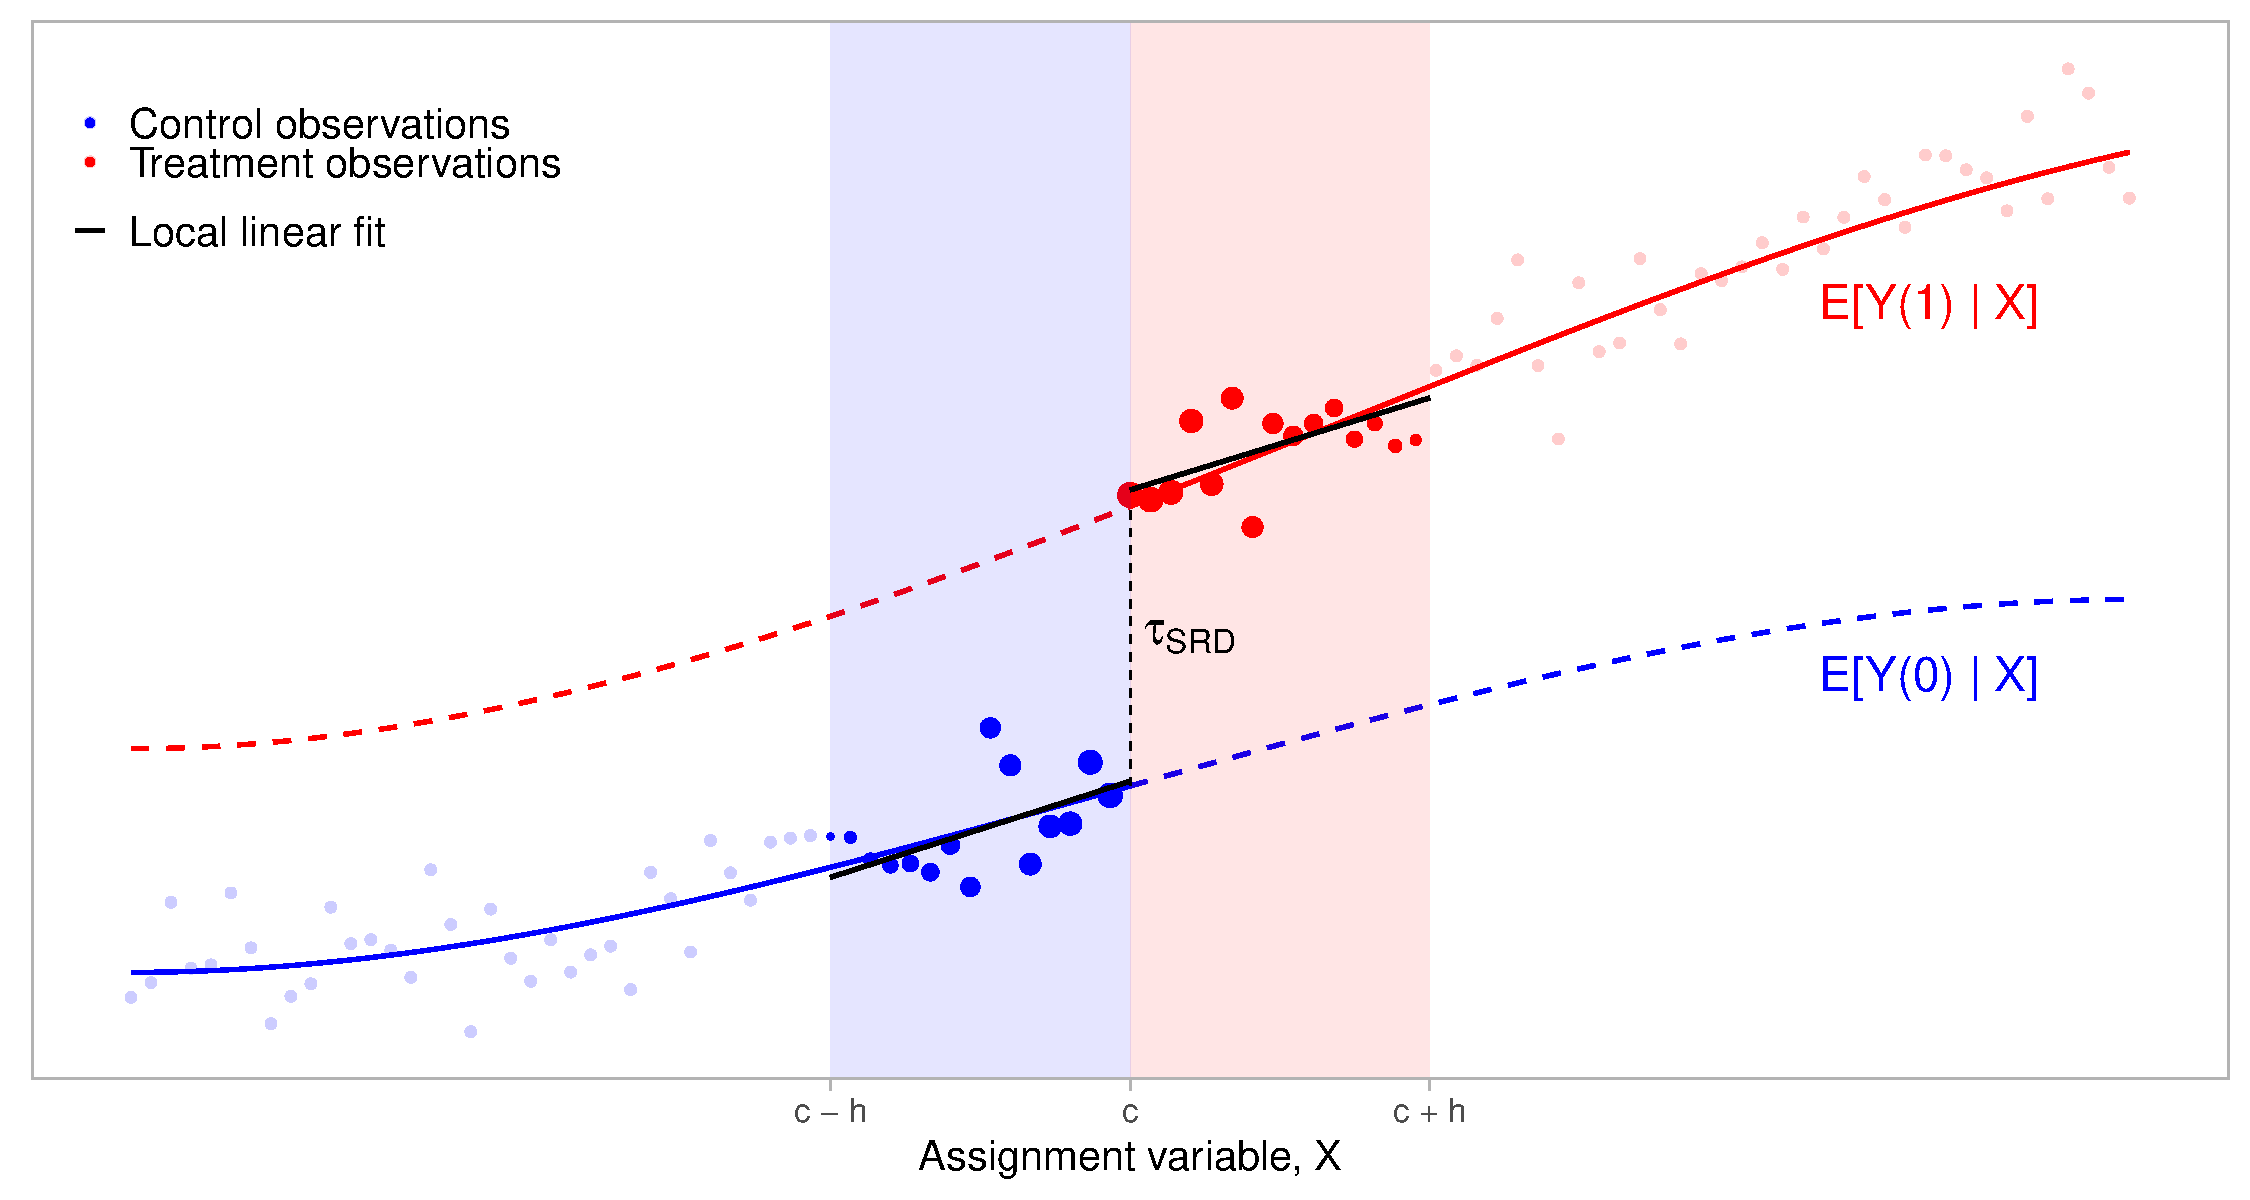
\includegraphics[width=\textwidth]{figure_03.pdf}
	\caption{Local linear estimation of the RD treatment effect $\tau_{\SRD}$.
			 Observed are random outcomes for the setting from Figure~\ref{fig:regression_functions_SRDD}.
		 	 The treatment effect is estimated by fitting locally a weighted linear regression, separately for control and treatment units.
	 	 	 The estimation windows, $[c - h, c]$ (control) and $[c, c + h]$ (treatment), are determined by the common bandwidth $h$.
 	 	 	 The weights, as given by the triangular kernel, are represented by the size of the dots in the shaded windows.}
	\label{fig:ll_estimation}
\end{figure}

\subsection{Bandwidth selection}

The bandwidth is referred to as the smoothing parameter.
Heuristically, a larger bandwidth leads to more (smoothing) bias, as the lower-order polynomial approximation of the unknown regression function near the cutoff gets worse.
At the same time, the variance of the estimator decreases, as more observations are used.
Analogously, a smaller bandwidth generally leads to less bias, but increased variance.
Therefore, the bandwidth selection involves a bias-variance trade-off.
In Figure~\ref{fig:ll_estimation} both functions are well approximated by a first-order polynomial in the respective neighborhood;
bias will be small.

An ad hoc way of choosing the bandwidth is by \enquote{eyeballing}.
However, RD estimation and inference results are sensitive to the bandwidth choice, requiring automatic, data-dependent procedures.
Two popular procedures are cross-validation (CV) and plug-in.
\textcite{Imbens_2008} proposed a version of CV specifically for the RD design, aimed at estimation at the boundary.
To obtain a bandwidth with higher accuracy near the cutoff,
it may be prudent to discard units far away from the cutoff before computing the CV criterion. 

The plug-in method for a common bandwidth consists of deriving an explicit formula for the bandwidth that minimizes an asymptotic approximation to the
mean squared error (MSE) of $\tauhatSRD$, and then to plug in estimators for the unknown quantities in this formula.
The asymptotic or leading (conditional) MSE of $\tauhatSRD$ is
\begin{equation}
	\AMSE(\tauhatSRD) = \ABias^2(\tauhatSRD) + \AVar(\tauhatSRD) \,.
\end{equation}
For the bias term it can be shown \parencite[Section~4.2.2]{Cattaneo_2020_book} that
\begin{equation} \label{eq:ABias}
	\ABias(\tauhatSRD) = h^{p+1} \mathcal{B} \,, 
\end{equation}
with
\begin{equation}
	\mathcal{B} = \mathcal{B}_\lowr - \mathcal{B}_\lowl \,,\quad \mathcal{B}_\lowl = \mu_\lowl^{(p+1)} B_\lowl \,,\quad \mathcal{B}_\lowr = \mu_\lowr^{(p+1)} B_\lowr \,,
\end{equation}
\begin{equation}
	\mu_\lowl^{(p+1)} \equiv \lim_{x \uparrow c} \frac{\diff^{p+1} \E[Y(0) | X = x]}{\diff x^{p+1}} \,,\quad  
	\mu_\lowr^{(p+1)} \equiv \lim_{x \downarrow c} \frac{\diff^{p+1} \E[Y(1) | X = x]}{\diff x^{p+1}} \,.
\end{equation}
The constants $B_\lowl$ and $B_\lowr$ depend on the chosen kernel $K$ and polynomial order $p$.
The derivatives are related to the approximation errors of the $p$th-order polynomial approximations.
For instance, in case of local linear regression the error is driven by the second derivative.
The error increases in the curvature of the regression function.
Notice that, if $\mu_\lowl^{(p+1)}$ equals $\mu_\lowr^{(p+1)}$, the bias term can be offset.\footnote{If $p$ is uneven (e.g.\ as in local linear estimation), then $B_\lowl = B_\lowr$. See \textcite[Lemma A.1]{Calonico_2014}.}
For the asymptotic (conditional) variance it can be shown that
\begin{equation} \label{eq:AVar}
	\AVar(\tauhatSRD) = \frac{1}{nh} \mathcal{V} \,, 
\end{equation}
with
\begin{equation}
	\mathcal{V} = \mathcal{V}_\lowl + \mathcal{V}_\lowr \,,\quad \mathcal{V}_\lowl = \frac{\sigma_\lowl^2}{f_X(c-)} V \,,\quad \mathcal{V}_\lowr = \frac{\sigma_\lowr^2}{f_X(c+)} V \,,
\end{equation}
\begin{equation}
	\sigma_\lowl^2 \equiv \lim_{x \uparrow c} \Var(Y(0) | X = x) \,,\quad  
	\sigma_\lowr^2 \equiv \lim_{x \downarrow c} \Var(Y(1) | X = x) \,,
\end{equation}
\begin{equation}
	f_X(c-) \equiv \lim_{x \uparrow c} f_X(x) \,,\quad  
	f_X(c+) \equiv \lim_{x \downarrow c} f_X(x) \,.
\end{equation}
The constant $V$ depends on the chosen kernel $K$ and polynomial order $p$.
The presence of the density of the assignment variable $f_X$ at the cutoff reflects that variance will be larger if fewer observations close to the cutoff are available.
Notice that due to local estimation the effective sample size is $nh$ and not $n$.

The bias-variance trade-off is formally expressed by the optimization problem
\begin{equation}
	\min_{h>0} \,\, \AMSE(\tauhatSRD) = h^{2(p+1)} \mathcal{B}^2 + \frac{1}{nh} \mathcal{V} \,.
\end{equation}
A smaller bandwidth leads to reduced bias, but larger variance, and vice versa.
The resulting (A)MSE-optimal bandwidth is
\begin{equation} \label{eq:hMSE}
	h_{\text{MSE}} = \left( \frac{\mathcal{V}}{2(p+1) \mathcal{B}^2} \right)^{1/(2p+3)} \cdot n^{-1/(2p+3)} \,.
\end{equation}
Thus, for the local linear estimator $h_{\text{MSE}} \sim n^{-1/5}$.
This bandwidth is not directly applicable, as several ingredients are unknown in practice and estimates need to be plugged in first.
The bias estimation is more involved.
Estimates of $\mu_\lowl^{(p+1)}$ and $\mu_\lowr^{(p+1)}$ are obtained by separate local polynomial regressions,
with polynomial order $q \geq p+1$ and preliminary bandwidth $b$.
This bandwidth often relies on a rule of thumb.
\textcite{Imbens_2012} were the first to implement a plug-in bandwidth selector according to \eqref{eq:hMSE}
by substituting consistent estimators, albeit for $p=1$ only.
The bandwidth selector of \textcite{Calonico_2014} instead applies for any $p$.
Besides, their selector improves on the estimation of the variance component $\mathcal{V}$ and how preliminary bandwidths are chosen.
Under standard assumptions, both estimators are consistent and optimal in the sense of \textcite{Li_1987}.
Also, in distinction to $h_{\text{MSE}}$, both incorporate a (positive) regularization term in the denominator
to adjust for potential low precision in estimating $\mu_\lowl^{(p+1)}$ and $\mu_\lowr^{(p+1)}$ \parencite[Section~4]{Imbens_2012}.
The motivation is that even when substantial curvature is present, due to low precision the estimated biases may be small,
resulting in a very large and poor-performing bandwidth.